Using 'typical' values for voice source parameters is hard because trans voices differ from typical male or female voices. \cite{Gunzburger1995} Particularly for trans women there is a tendency for $F_3$ to be raised compared to male voices, with slower speech at reduced loudness and a higher $F_0$. 

Although the implementation of the LF-model is there I had difficulty utilising it to improve my synthesiser. Determining correct parameters is not trivial as using this `analysis-by-synthesis' approach to compare the synthesised spectrogram with the reference requires a lot of time in a non-automated system such as this PD implementation.

The additional parameters in the revised model \cite{Fant1995} provide further control over the spectrum: increasing $R_k$ raises level of voice fundamental relative to upper parts of the spectrum. Increasing $R_g$ promotes the level of the second harmonic at the expense of the fundamental. This analysis starts to get into the spectral qualities of specific voices, e.g. it is noted that sonorous voices have relatively high $F_a$ of the order of \si{2000Hz} \cite{Fant1995}.

Fant also discusses a shape parameter, $R_d$, which predicts the other values, citing a 1994 publication that I was unable to locate a copy of \cite{Fant1994}. I tried to implement this as I felt it would make it much more straightforward to find appropriate LF-model parameters for my system, however I had enormous problems matching up the ``statistical relations" for the R parameters in the LF-model \cite{Fant1995} - particularly due to an initial misunderstanding of the statistical prediction model. The work in progress for this can be seen in the \obj{lfmodel\char`~} patch. I would very much like to do more research into this and complete the revisited model.

I found that much of my alterations, though making sense from a theoretical perspective and being audible in contrived examples, made minimal impact when real words were being synthesised. It's probably quite important to do real listening tests.

One issue with my system is that the transitions between parameters, e.g. formant centre frequencies, are linear. This isn't actually true to formants in actual speech which have more gradual ramps between positions. See Figure \ref{fig:bout_non_linear_tx} below for an example in an earlier word. For my final word I compensated for this somewhat by having more interpolation points during the word and ramping between them. 
%
\begin{figure}[H] 
	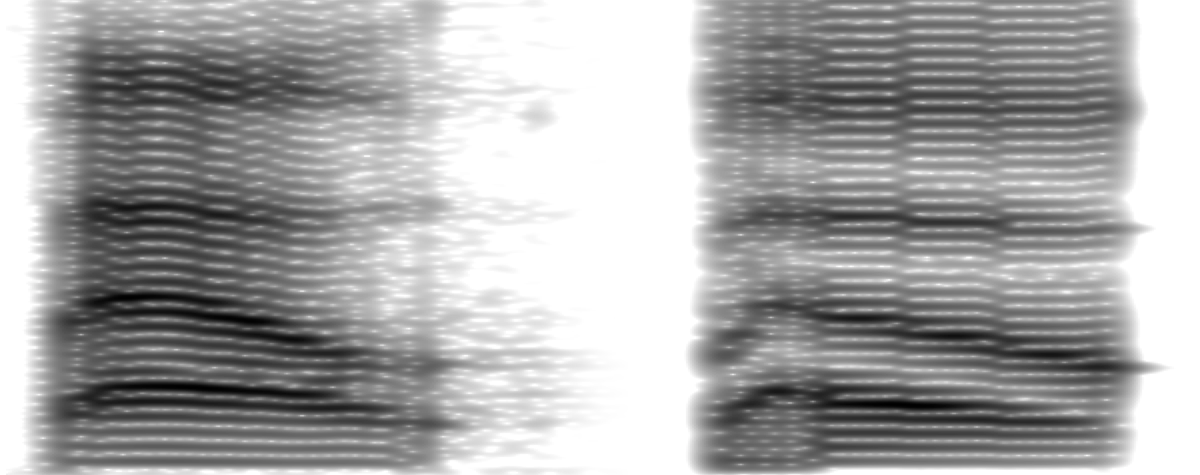
\includegraphics[width=0.5\textwidth]{bout_non_linear_tx.png}
	\caption{Linear vs. non-linear formant transitions of \ipa{baʊt} in the reference recording (left) vs synthesised (right).}
	\label{fig:bout_non_linear_tx}
\end{figure}
%
One compromise I made was to have frication noise production independent of the LF model. In the human vocal tract, the jet stream is interrupted when the glottis is closed. This is why voiced consonants have less power than unvoiced. To implement this I would need to integrate the glottal derivative to get the actual glottal flow, and amplitude modulate the frication noise with this signal. I'm not sure to what extent the difference would be perceptible, but it would perhaps make it easier to get the power of the voiced vs unvoiced source correctly distributed for mixed phonemes. Another choice that may have made the model more helpful was if the frication noise bypassed the formants altogether or used a different formant chain. This is because the `sound source' for fricatives is not the glottis but rather the area where the jet stream hits a wall, e.g. the teeth, although the vocal tract does modulate the power that this source receives. Filtering this signal through the vocal tract is therefore removing a lot of the signal that shouldn't be filtered. I compensated for this somewhat by setting the bandwidth of the formants widely.

A problem with my LF-model is that when parameters are adjusted it will rewrite the glottal derivative waveform once per DSP cycle (as soon as one parameter is updated it blocks all others until that rewrite is complete).

This would be fine if it could update the glottal waveform in one DSP cycle (approximately 23µs per cycle). When I timed the calculation on my machine it took 1310µs to complete a cycle which is a significant loss of resolution.

A better solution might be to continually update the glottal waveform, in this case interpolation would need to be done between values to prevent introducing a lot of high frequency distortion when the time-domain amplitude changes rapidly based on a completely different glottal derivative (this effect is somewhat masked by the per-cycle update because the glottal waveform tends to gravitate towards zero at the start and end of the cycle).

An alternative to the LF-model has been proposed that is more computationally efficient and demonstrated to be perceptually equivalent in a psychoacoustic experiment \cite{Veldhuis1998}. In order to move the system towards real-time manipulation of the glottal derivative, and or to increase the sample rate, this could be useful to implement.

Sometimes there is interpolation noise/distortion which really is unacceptable and should be eliminated although because PD can be somewhat obtuse in the order it processes things and the timings of commands being sent this can be somewhat difficult.

One problem was that the more control parameters were added to the synthesiser the harder it got to experiment to find the right sound (partially down to a bug in OS X PD where the typing caret does not appear in message boxes). At the start it was much easier to pin down a certain sound before more 'realistic' parameters were added and iteration became much slower.

Can show waveforms of my voice vs. what comes out of the synthesiser. Note it would be nice to be able to record the voice things with an extremely flat microphone at consistent distances with measured freq responses in an anechoic chamber for proper comparison (and normalize the levels).

There's a few things I attempted to develop in this project but that I had trouble with that would be potential room for development. I spent a lot of time researching voice source models to try and build a system that could produce characteristic sound of a human voice. Part of this voice source model involves the voice source parameters changing in response to certain things. For example the acoustic characteristics of the source in one vowel may be different to another, or for consonants, or even due to stress, loudness, tiredness, and endless other factors. Although I did try implementing a system that boiled down, using statistical relations, the voice source parameters for various vowels, I did not manage to get it working due to time and availability constraints. 
This could form part of a large system that would allow the modulation of the voice in terms of emotion, stress, and prosody.
To get an accurate set of voice source parameters I could use inverse filtering to negate the effects of the vocal tract on a voice recording, although it may be difficult to reproduce sound precisely with the LF-model and this approach due to recurrent patterns and randomness in normal human speech \cite{Fant1995}.

I would like to implement a complete set of IPA phonemes in the synthesiser. For the most part this would be as simple as analysing them in Praat and keying the values into the synthesiser. For some types of consonants this would be more complicated. It seems like an optimised synthesiser would allow automated targeting of speech and would try and fit the parameters to this as best as possible.

The noise for the fricatives just uses PD's \texttt{pink~} object. Whilst this is more realistic than white noise it doesn't quite share the same spectral properties as the fricative noise actually produced by the body \cite{Johnson2003}. It would be good to create a more sophisticated model of the source of unvoiced sounds such as there is for voiced sounds.

A more sophisticated model for future implementation could use a physical model which mimics the details of the glottal excitation process \cite{Liljencrants1995}. It would be important to determine however that the difference is perceptible.

It has been demonstrated that there's an association between excitation amplitude $E_e$ with $F_0$ in Swedish. \cite{Fant1994}. Assuming this extends to English, it could be a factor for an improved system that can convey some more extra-lingual semantics onto the speech synthesis system, e.g. making the synthesised speech sounding more stressed.

discuss bandwidth of formants not showing much affect on naturalness perception

discuss relatively cumbersome development process in PD vs other processes

limitations of building phoneme by phoneme. success for single words but more involved in full sentences

Additional features such as vocal fry would require more work. \cite{Gobl1988} states glottal flow for creaky phonation differing substantially.

\cite{Klatt1990} states transition from a voiceless consonant to a vowel often includes a short interval of breathy voicing in which the first-harmonic amplitude is increased. This could indicate the need to add aspiration noise as well as adjust the voice source parameters to increase the first-harmonic.

\cite{Klatt1990} notes that breathiness increases for unstressed  and final syllables, and at the margins of voiceless consonants.

\cite{Klatt1990} also discusses scenarios where different formant models, cascade or parallel, are applicable, and amplitude modulation of aspiration and frication noise to simulate the effect of vocal-fold vibration:

".
There is a cascade formant model
of the vocal-tract transfer function for laryngeal sound sources,
and a parallel formant model with formant ampli-
tude controls for frication excitation.
A third vocal-tract
model in which the vocal-tract transfer function for laryn- geal sound sources
is approximated by formants
configured
in parallel is useful for some specialized
synthesis
applica-
tions, but is normally not used.
As was the case in the origi-
nal formant synthesizer,
the aspiration and frication noise
sources are amplitude modulated, to simulate the effect of vocal-fold vibration, if AV is nonzero."

Would probably reimplement in something like Super collider but if had to continue using PD would work more on control primitives so that prototyping is much faster.

As it was not implemented fully in my final design I have removed the details from this report 

The 'shape parameter' $R_d = (U_0/E_e)(F_0/110)$.  \cite{Fant1995} discusses some statistical relations, cited from  a 1994 publication that I was unable to locate a copy of. \cite{Fant1994}. These are the following predicated values, as they relate to $R_d$, and an estimation of $R_d$ from the geometrical constraints of the LF model:

\begin{align}
R_a & \approx (-1+4.8R_d)/100 \\
R_k  & \approx (22.4 + 11.8R_d)/100 \\
R_d & \approx (1/0.11)(0.5+1.2R_k)(R_k/4R_g+R_a)
\end{align}
The main range of variation is $0.3 < R_d < 2.7$, and the upper range is intended for transitions towards complete abduction as in prepause voice terminations.

Here's an example of the variation from \cite{Fant1995}: "
A pronounced vocal-tract narrowing, as in the [i:] and [y:] and the maximally rounded [u:] and [\sout{u}:], causes a loss of transglottal pressure which modifies the glottal flow pulse towards a greater $R_d$ value and a somewhat lower $E_e$."

Higher $R_d$ is typical of female vs male phonations, but also found in voiced consoants and aspirated vowels vs regular vowels. \cite{Fant1995}

Klatt \cite{Klatt1990} discusses a diplophonic double pulsing in whcih pairs of glottal pulses migrate toward one another and the first of the pair is usually attenuated in amplitude. Tends to occur when the fundamental is low (voicing is unstable). (possible further improvement).

Found consonans hadest. \cite{Johnson2003} notes that it is harder to measure acoustic characteristics of fricatives because there may be several spectral peaks which change relative amplitude from one utterance to another

